\section{System Model}
%\subsection{Task Model}
\subsection{Communication Model}
\subsection{Computation Model}

\begin{frame}
	\frametitle{System Model}


\textbf{We consider}

\vspace{2mm}

	\begin{itemize}
		
		\item the set of MD $\mathcal{I} = \{1, 2, ..., I\}$ 
		
		\vspace{2mm}
		
		\item the set of EN $\mathcal{J} = \{1, 2, ..., J\}$
		
		\vspace{2mm}
		
		\item set of time slots $\mathcal{T} = \{1, 2, \ldots, T\}$
		
		\vspace{2mm}
		
		\item each MD $i \in \mathcal{I}$ are connected to each EN $j \in \mathcal{J}$ with it's wireless interface. 		
		
		\vspace{2mm}
		
		
		\item each time slot consider as a diuration of time. 
		
	\end{itemize}
	
\end{frame}

\begin{frame}
	\frametitle{System Model}
	
	\begin{figure}
		\captionsetup{name=Fig.}
		\centering
		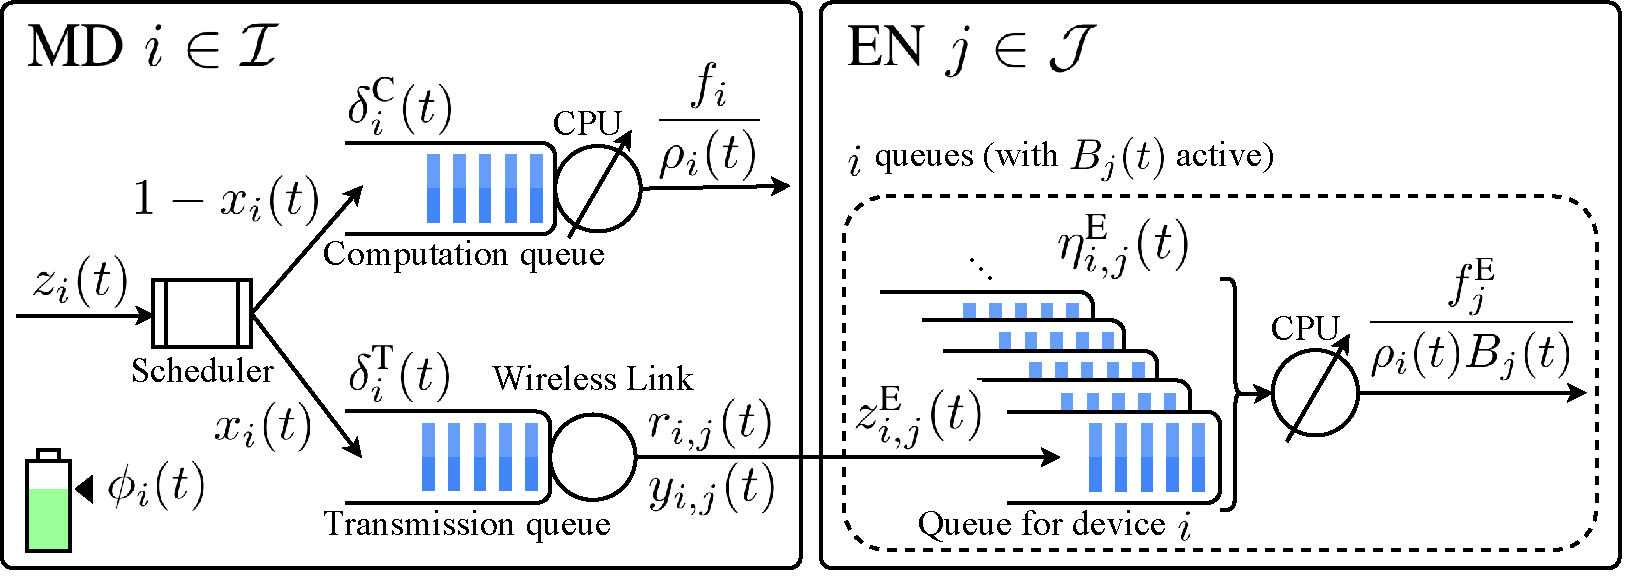
\includegraphics[width=1\linewidth]{queue}
		\vspace*{-5mm}
		%\caption{An illustration MD $i \in \mathcal{I}$ and EN $j \in \mathcal{J}$ in the MEC system.}
		\vspace*{-3mm}
		\label{fig1}
	\end{figure}

\vspace{2mm}
	\vfill
	\textbf{Task}\vspace{2mm}

	\begin{enumerate}[$\bullet$]
	
	\item $z_i(t)$:  arrived task in MD
	\item 	$\lambda_i(t)$:  Required CPU cycles of task 
	\item $\rho_i(t)$:    Required CPU cycles of task 
	\item $\Delta_i(t)$:   Required CPU cycles of task

	
	\end{enumerate}

\end{frame}

\begin{frame}
	\frametitle{System Model}
	
	\begin{figure}
		\captionsetup{name=Fig.}
		\centering
		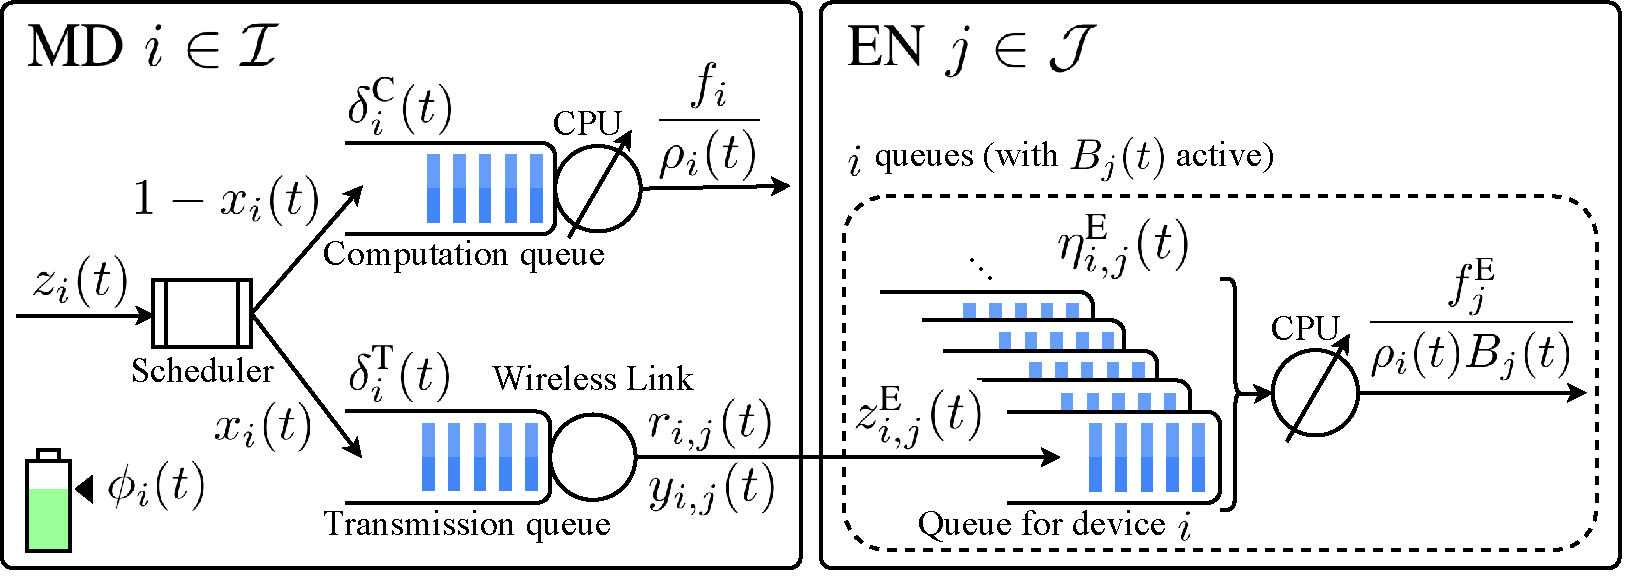
\includegraphics[width=1\linewidth]{queue}
		\vspace*{-5mm}
		%\caption{An illustration MD $i \in \mathcal{I}$ and EN $j \in \mathcal{J}$ in the MEC system.}
		\vspace*{-3mm}
		\label{fig1}
	\end{figure}
	
	\vfill
	
	\textbf{Offloading}\vspace{2mm}
	
	\begin{enumerate}[$\bullet$]
		
		\item $x_i(t)$:    Offloading Decision 
		\item $y_{i,j}(t)$:   Offloading Target  
		
	\end{enumerate}


\end{frame}



\begin{frame}
	\frametitle{System Model}
	
	\begin{figure}
		\captionsetup{name=Fig.}
		\centering
		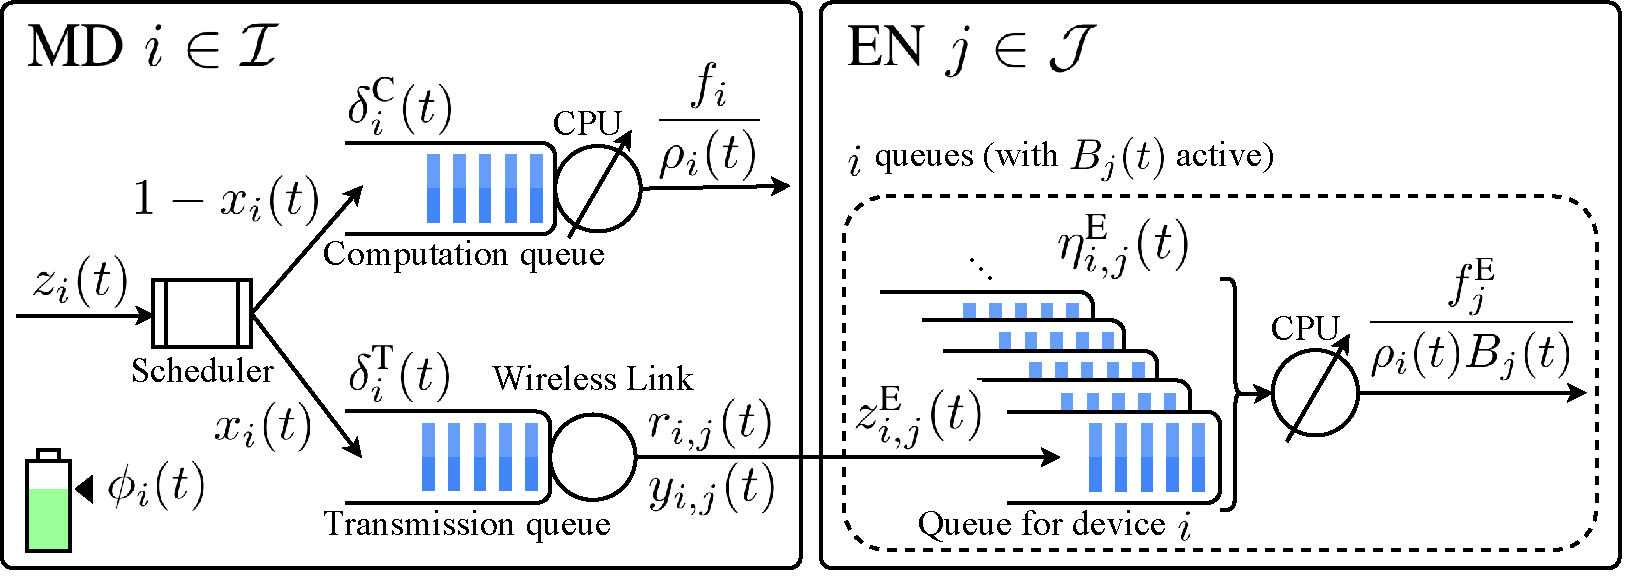
\includegraphics[width=1\linewidth]{queue}
		\vspace*{-5mm}
		%\caption{An illustration MD $i \in \mathcal{I}$ and EN $j \in \mathcal{J}$ in the MEC system.}
		\vspace*{-3mm}
		\label{fig1}
	\end{figure}
	
	\vfill
	
	\textbf{Queues' Information}\vspace{2mm}
	
	\begin{enumerate}[$\bullet$]
		
		\item $\delta^C_i(t)$  Compution Queue in MD
		\item $\delta^T_i(t)$  Transsmition Queue in MD
		\item $\eta^E_{i,j}(t)$  MD Compution Queue in EN
		
	\end{enumerate}
	
%				$f_i$  &  Computation capacity of MD \\
%$f_j^{E}$ & Computation capacity of EN\\ 
%$\phi_i(t)$ & MD battery level\\
%$r_{i,j}(t)$ &  Transmission capacity of MD \\
%$\eta^E_{i,j}(t)$ &  MD Compution Queue in EN\\
%$\eta^E_{i,j}(t)$ &  MD Compution Queue in EN\\
%$B_j(t)$ & Active Queue in EN
	
\end{frame}



\begin{frame}
	\frametitle{Communication Model}

	\vspace{2mm}

		\begin{itemize}[]

		\item $\delta_i^{T}(t)$: MD $i$ \textcolor{teal}{Transmission Queue Waiting Time}%to represent the time slot when the task is either dispatched to the EN or dropped: 
		\vspace{-3mm}
		\begin{alignat}{2}
			\delta_i^{T}(t) = \left[\max\limits_{t^{'}\in  \{0,1,\ldots,t-1\}} l_i^{T}(t^{'})-t+1\right]^+
			\label{1}  
		\end{alignat}
		
		
		\item $l_i^{T}(t)$: \textcolor{teal}{Task Transmited/Dropped Time Slot}
		\begin{alignat}{2}
			l_i^{T}(t) = \min \Big\{t + \delta_i^{T}(t) + \lceil{D_i^{T}(t)}\rceil - 1, t + \Delta_i(t) - 1\Big\}
			\label{2}  
		\end{alignat}
		
		
		\item $D_i^{T}(t)$:	\textcolor{teal}{Task Transmission Time}
		\vspace{-4mm}
		\begin{alignat}{2}
			D_i^{T}(t) =  \sum_{\mathcal{J}} y_{i,j}(t) {\lambda_i(t) \over r_{i,j}(t)\tau}
			\label{3}  
		\end{alignat}
	
		
		
		\item $E_i^{T}(t)$:	\textcolor{teal}{Task Transmission Energy Consumption}
		\vspace{-1mm}
		\begin{alignat}{2}
			E_i^{T}(t) = D_i^{T}(t)p_i^{T}(t)\tau
			\label{4}  
		\end{alignat}

	
	\end{itemize}
\end{frame}


\begin{frame}
	\frametitle{Computation Model}
	\textbf{Local Execution:}
	
	\vspace{2mm}
	
	\begin{itemize}[]
		
		\item $\delta_i^{C}(t)$:  \textcolor{teal}{MD $i$ Computation Queue Waiting Time}%to represent the time slot when the task is either dispatched to the EN or dropped: 
		\vspace{-3mm}
		\begin{alignat}{2}
			\delta_i^{C}(t) = \left[ \max \limits_{t' \in \{0,1,\ldots,t-1\}} l_i^{C}(t')-t+1 \right]^+
			\label{5}  
		\end{alignat}
		
		
		\item $l_i^{C}(t)$: \textcolor{teal}{Task Executed/Dropped Time Slot}
		\begin{alignat}{2}
			l_i^{C}(t) = \min \Big\{t + \delta_i^{C}(t) + \lceil D_i^{C}(t) \rceil - 1, t + \Delta_i(t) - 1\Big\}
			\label{6}  
		\end{alignat}
		
		
		\item $D_i^{C}(t)$:	\textcolor{teal}{Task Execution Time}
		\vspace{-4mm}
		\begin{alignat}{2}
			D_i^{C}(t) = { \lambda_i(t)  \over  f_i  \tau /  \rho_i(t)}
			\label{7}  
		\end{alignat}
		
		
		
		\item $E_i^{L}(t)$:	\textcolor{teal}{Task Execution Energy Consumption}
		\vspace{-1mm}
		\begin{alignat}{2}
			E_i^{L}(t) =  D_i^{C}(t) p_i^{C}  \tau %=  { \lambda_i(t) \rho_i(t)  \over  f_i} p_i^{\text{C}},
			\label{8}  
		\end{alignat}
		
		
	\end{itemize}
\end{frame}


\begin{frame}
	\frametitle{Computation Model}
	\textbf{Edge Execution:}
	
	\vfill
	
	\begin{itemize}[]
		

		
		
		\item $\eta_{i,j}^{E}(t)$: \textcolor{teal}{MD $i$ Queue Backlog at EN $j$}
		\vspace{-2mm}
		\begin{alignat}{2}
				\eta_{i,j}^{E}(t)=\left[\eta_{i,j}^{E}(t-1)+\lambda_{i,j}^{E}(t)-{f_j^{E}\over \rho_i(t)B_j(t)} -\omega_{i,j}(t)\right]^+\hspace{-1.7mm}
			\label{10}  
		\end{alignat}
	
		\item $\hat{l}_{i,j}^{E}(t)$: \textcolor{teal}{Task Execution Start Time Slot at EN $j$}
		\vspace{-2mm}
		\begin{alignat}{2}
			\hat{l}_{i,j}^{E}(t) = \max \{t, \max \limits_{t^{'} \in \{0,1,\ldots,t-1\}} l_{i,j}^{E}(t^{'})+1\}
			\label{11}  
		\end{alignat}
			\vspace{-4mm}
		\begin{alignat}{2}
				\sum_{t^{'}=\hat{l}_{i,j}^{E}(t)}^{l_{i,j}^{E}(t)}{f_j^{E} \over \rho_i(t)B_j(t^{'})}  \geq   \lambda_{i,j}^{E}(t) > \sum_{t^{'}=\hat{l}_{i,j}^{E}(t)}^{l_{i,j}^{E}(t)-1}{f_j^{E} \over \rho_i(t)B_j(t^{'})} 
				\label{12} 
		\end{alignat}
		
		

		
	\end{itemize}
\end{frame}


\begin{frame}
	\frametitle{Computation Model}
	\textbf{Edge Execution:}
	
	\vfill
	
	\begin{itemize}[]
		
				\item $D_{i,j}^{E}(t)$:	\textcolor{teal}{Task Execution Time at EN $j$}
		\vspace{-2mm}
		\begin{alignat}{2}
			D_{i,j}^{E}(t) = { \lambda_{i,j}^{E}(t) \rho_i(t) \over f_j^{E} \tau /  B_j(t)}
			\label{14}  
		\end{alignat}
		
		
		
		\item $E_{i,j}^{E}(t)$:	\textcolor{teal}{Task Execution Energy Consumption at EN $j$}
		\vspace{-2mm}
		\begin{alignat}{2}
			E_{i,j}^{E}(t) = {D_{i,j}^{E}(t)  p_j^{E} \tau \over B_j(t)}  % = { \lambda_{i,j}^{\text{E}}(t) \rho_i(t) \over  f_j^{\text{E}}}p_j^{\text{E}} ,
			\label{15}  
		\end{alignat}
		
		\item $E_i^{I}(t)$:	\textcolor{teal}{MD $i$ Standby Energy Consumption} 
		\begin{alignat}{2}
			E_i^{I}(t) = D_{i,j}^{E}(t) p_i^{I} \tau%= {\lambda_{i,j}^{\text{E}}(t) \rho_i(t) \over \mathcal{B}_j(t) f_j^{\text{E}}} p_i^{\text{I}},
			\label{16}
		\end{alignat}
	
		\item $E_i^{O}(t)$: \textcolor{teal}{Overall Offloading Energy Consumption}
		\begin{alignat}{2}
			E_i^{O}(t) = E_i^{T}(t) + \sum_{\mathcal{J}} E_{i,j}^{E}(t) + E_i^{I}(t).
			\label{17}
		\end{alignat}
		
		


	\end{itemize}
\end{frame}
